\begin{minipage}{0.4\linewidth}
    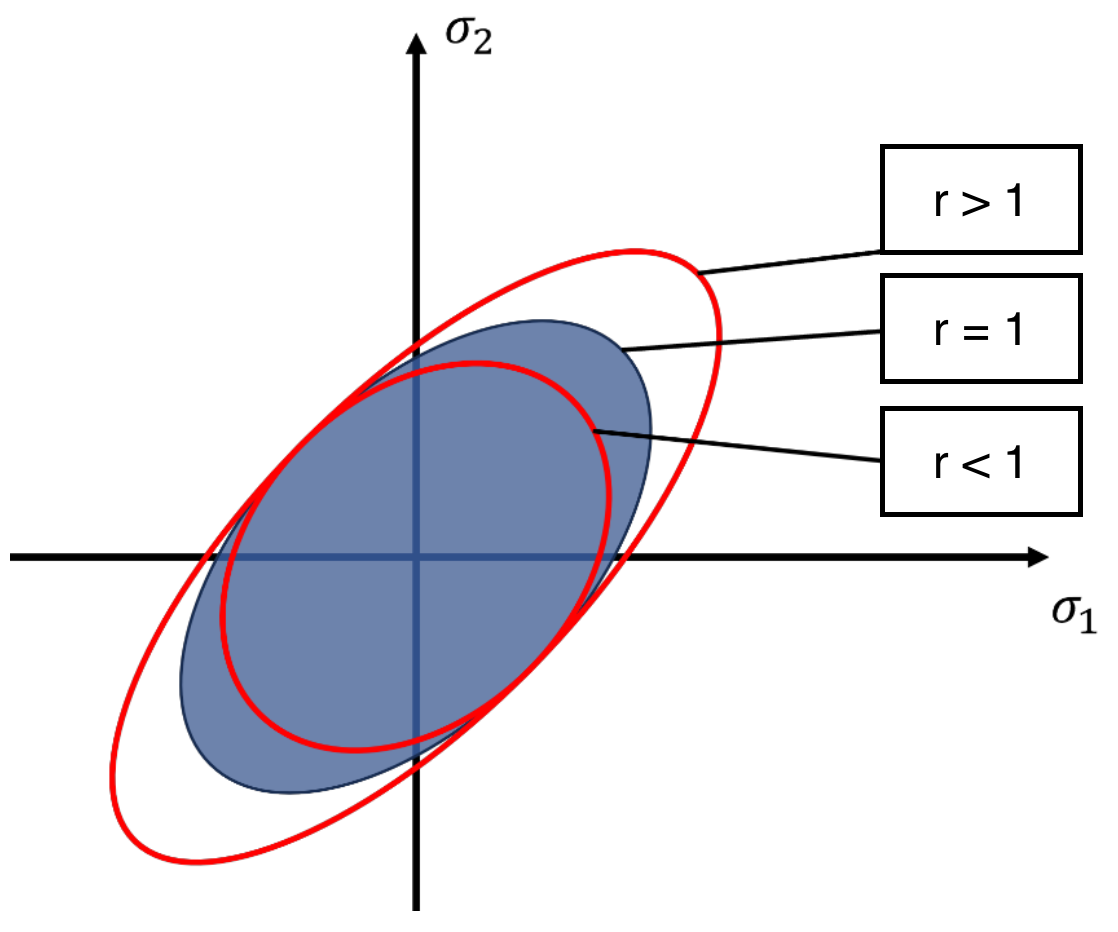
\includegraphics[width = 0.9\linewidth]{src/images/Isotropie.png}
    \mathbox{
        r = \frac{\sigma_2}{\sigma_1}
    }
\end{minipage}
\begin{minipage}{0.6\linewidth}
    \textbf{Isotropisches} Material verformt sich in 
    alle Richtungen gleich gut.\\
    r = 1\\

\textbf{Anisotropisches} Material verformt 
sich in verschiedene Richtungen unterschiedlich 
gut.\\
r $>$ 1 $\downarrow$ Dickenänderung, $\uparrow $ Breitenänderung (weniger Rissbildung)\vspace{1mm}\\
r $<$ 1 $\uparrow$ Dickenänderung, $\downarrow$ Breitenänderung
\end{minipage}
\vspace{1mm}\

Ebene Anisotropie:
Richtungsabhängigkeit der mechanischen Eigenschaften in einer Ebene.\\ 

Senkrechte Anisotropie:
Richtungsabhängigkeit der mechanischen Eigenschaften senkrecht zur Ebene.\\